\documentclass{suturo}
\usepackage{caption}
\begin{document}
    \maketitle{Motion}{09.03.2018}{}{1}{}{}{}{}

\makeatletter
\newcommand{\chapterauthor}[1]{%
  {\parindent0pt\vspace*{-27pt}%
  \linespread{0}\small\begin{flushright}von: #1\end{flushright}%
  \par\nobreak\vspace*{0pt}}
  \@afterheading%
}
\makeatother

\newpage
\section{Node: main (motion\_suturo\_1718)}
\subsection{Architekturbild}
\chapterauthor{Roman Haak}
\begin{figure}[!htb]
        \center{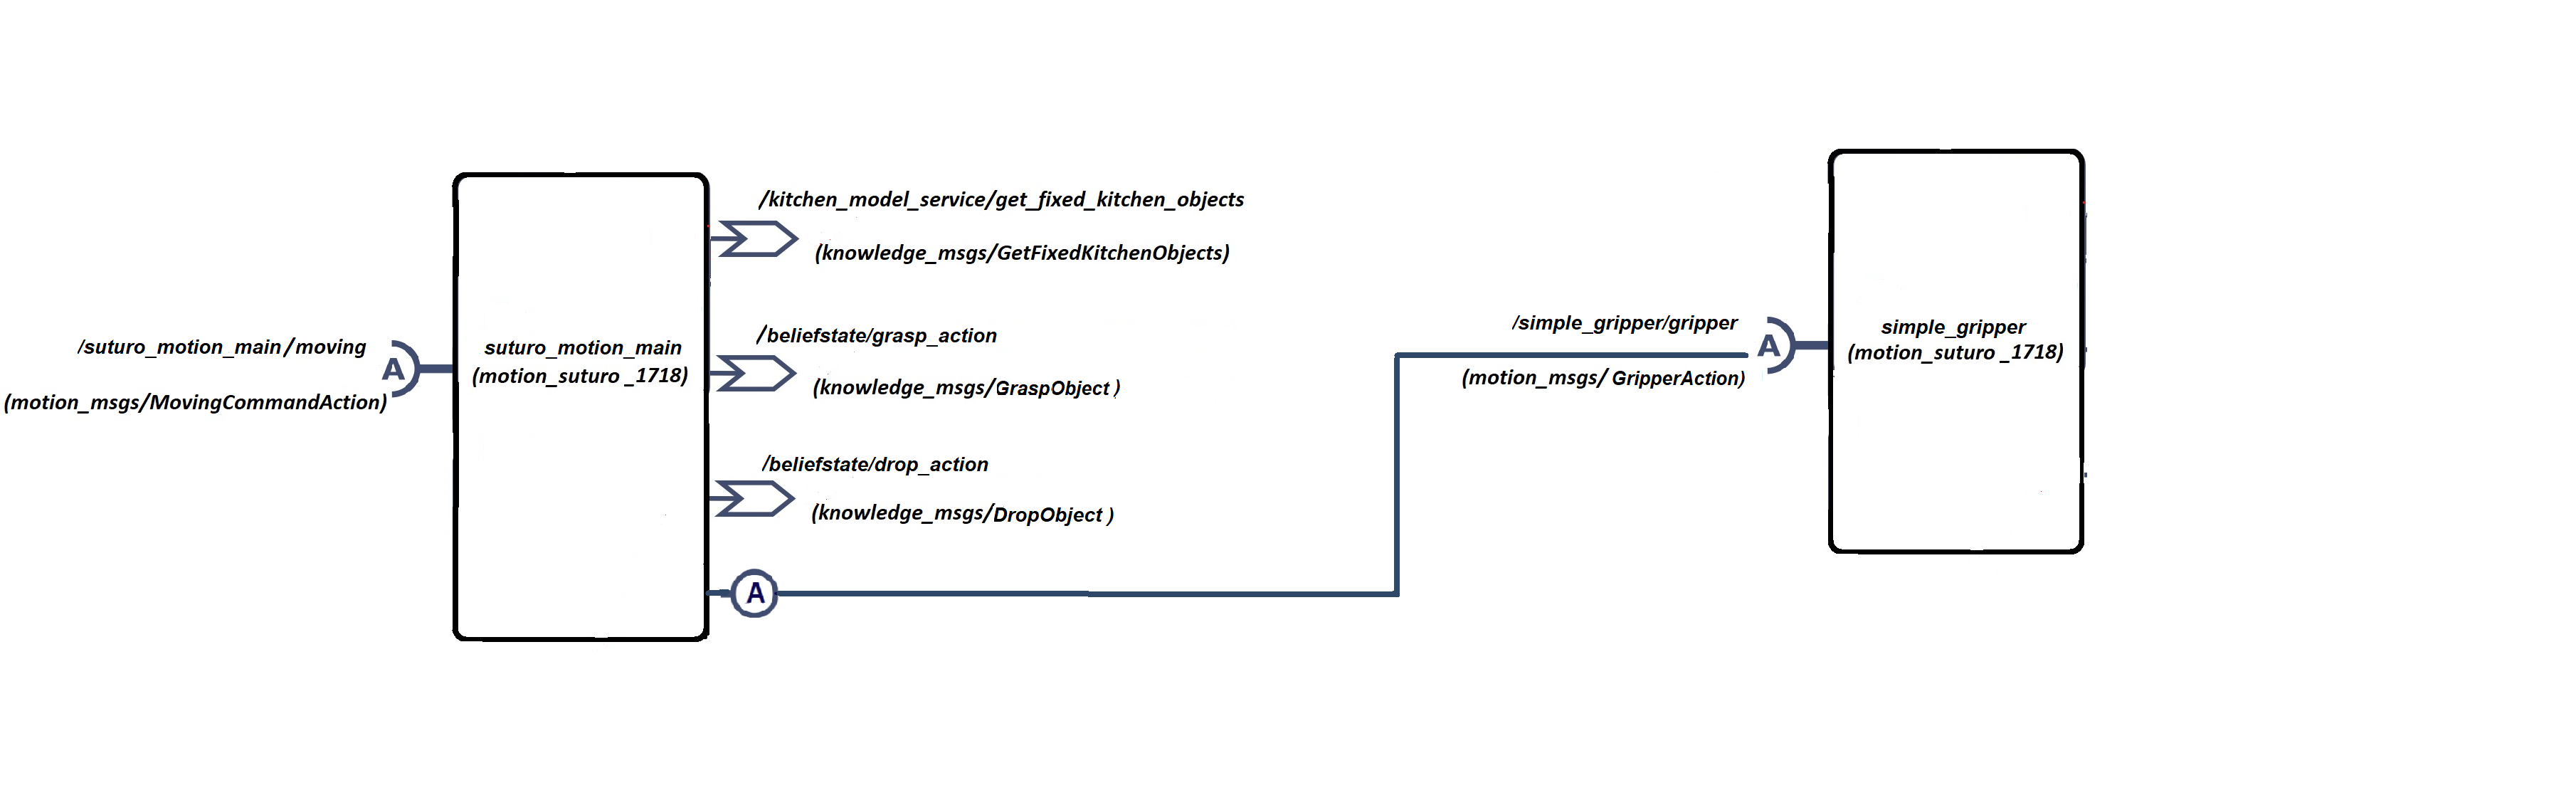
\includegraphics[width=\textwidth]
        {img/Architekturbild.png}
        \caption{\label{fig:motion_node} Architektur der motion-node}}
\end{figure}

\subsection{API}
\subsubsection{Serviceclient}
\chapterauthor{Roman Haak}
'\textit{/kitchen\_model\_service/get\_fixed\_kitchen\_objects}': \\
Dieser Service wird beim Initialisieren unseres Programms aufgerufen. Hierüber werden die Abmessungen der Objekte der IAI-Küche in die \textit{PlanningScene} geladen, damit der Roboter sich nur kollisionsfrei bewegt(siehe \textit{Kapitel 1.2.2}, Abschnitt zur '\textit{planning\_scene}').\\
Die Objekte sind dabei durch eine Höhe, Breite und Länge als \textit{Box-Collider} definiert.

\newpage
\subsubsection{Message Definitionen}
\chapterauthor{Maximilian Bertram}
'\textit{/motion/moving}': \\
Vom Typ '\textit{motion\_msgs/MovingCommand}': \\
\begin{lstlisting}[caption={Definition der MovingCommandAction},captionpos=b]
#goal definition
geometry_msgs/PointStamped point_stamped
uint8 command
#Constants for command value
uint8 UNKNOWN=0
uint8 MOVE_STANDARD_POSE=1
uint8 MOVE_RIGHT_ARM=2
uint8 MOVE_LEFT_ARM=3
uint8 MOVE_RIGHT_GRIPPER=4
uint8 MOVE_LEFT_GRIPPER=5
---
#result definition
bool successful
uint8 status
#Constants for status value
uint8 SUCCESS=0
uint8 OUT_OF_RANGE=1
uint8 COLLISION=2
uint8 UNMANAGEBLE_ERROR=3
---
#feedback definition
#bool finished
\end{lstlisting}
TODO: Namen?\\
'\textit{/motion/moving}': \\
Vom Typ '\textit{motion\_msgs/MovingCommand}': \\
\begin{lstlisting}[caption={Definition der GripperAction},captionpos=b]
#goal definition
#position of the space between the grippers in meters
float64 position
#force in newton (default =  20)
float64 effort
#which grpper to open/closed
uint8 gripper
#Constants for the gripper value
uint8 UNKNOWN=0
uint8 LEFT=1
uint8 RIGHT=2
---
#result definition
bool successful
---
#feedback definition
#bool finished
\end{lstlisting}




\subsection{Beschreibung des Teilsystems}
\subsubsection{Übersicht}
\chapterauthor{}

\subsubsection{Klassenvariablen}
\chapterauthor{}



\subsection{Programmablauf}
\chapterauthor{}

\subsubsection{Besonderheiten/Besondere Algorithmen}
\chapterauthor{}


\end{document}
